\documentclass[10pt,a4paper]{article}
\usepackage[utf8]{inputenc}
\usepackage[T1]{fontenc}
\usepackage{newtxtext,newtxmath}
\usepackage[brazil]{babel}
\usepackage{geometry}
\geometry{top=3.3cm,bottom=4cm,left=3cm,right=2.5cm}
\usepackage{graphicx,booktabs,array,tabularx,microtype}
\usepackage[authoryear,round]{natbib}
\usepackage[hidelinks]{hyperref}
\usepackage{titlesec}
\usepackage{caption}
\captionsetup{font=small,labelfont=bf}
\titleformat{\section}{\bfseries\normalsize}{\thesection.}{0.5em}{\MakeUppercase}
\titleformat{\subsection}{\bfseries\normalsize}{\thesubsection}{0.5em}{}
\titlespacing*{\section}{0pt}{1.2ex}{0.7ex}
\titlespacing*{\subsection}{0pt}{1ex}{0.5ex}
\setlength{\parindent}{0.55cm}
\setlength{\parskip}{0pt}
\setlength{\emergencystretch}{2em}
\pagestyle{empty}

\newif\ifcameraReady
\cameraReadyfalse
\newcommand{\repoReg}{\url{https://github.com/ReginaldoArakaki/PCS5039_ambiente_reg10k_vCl0}}
\newcommand{\repoArt}{\url{https://github.com/ReginaldoArakaki/PCS5039_reg10k_artigo-reprodutibilidade}}

\title{\vspace{-1.2cm}\bfseries\large DA AUTOMAÇÃO IoT ISOLADA À PLATAFORMA ORIENTADA A EVENTOS: UM LABORATÓRIO REPRODUZÍVEL DE DIGITAL TWINS NA PÓS-GRADUAÇÃO}
\author{\ifcameraReady Reginaldo Arakaki et al.\\Universidade de São Paulo\else Autores omitidos para revisão cega\fi}
\date{}

\begin{document}
\maketitle
\vspace{-1.2cm}

\begin{abstract}
Este artigo apresenta a evolução de um kit de automação residencial de iluminação para um laboratório reproduzível de arquitetura IoT orientada a eventos e integrado a Digital Twins. O artefato foi empregado na disciplina de pós-graduação PCS5039 para provocar decisões sobre percepção, conectividade, estado, comportamento e qualidade arquitetural. Três versões observadas ampliam o ambiente de um para quatro cômodos; uma quarta, planejada, desloca o foco para ocupação múltipla e intenção. O protocolo reúne 5.580 execuções, 2.790 pares controlador--cenário--semente, sete famílias de cenários e medidas de requisitos, energia, conforto, atualidade e fidelidade do gêmeo. Na V2, o controlador alternativo reduz desperdício em 12,37 s (IC95: $-26{,}75$; $-2{,}07$), mas aumenta o tempo no escuro com ocupante em 1,41 s (IC95: 1,02; 1,85). O erro de percepção domina o erro de sincronização no modelo simulado. Código, versões, massas e análises são identificados por repositório, tag, commit e manifesto. A contribuição é um instrumento de ensino e experimentação que torna explícito o percurso entre automação local, processamento de eventos, representação digital e serviços de plataforma, sem confundir viabilidade técnica com evidência causal de aprendizagem.

\textbf{Palavras-chave:} Internet das Coisas; Digital Twin; processamento de eventos complexos; arquitetura de sistemas; ensino de engenharia de software; reprodutibilidade.
\end{abstract}

\section{Introdução}

Uma automação de iluminação pode parecer um problema encerrado: detectar presença, decidir e acionar uma lâmpada. Essa formulação, porém, oculta as perguntas que surgem quando residências são conectadas. O sistema sabe que existe alguém parado ou apenas deixou de receber movimento? Distingue uma pessoa lendo de outra dormindo? Preserva decisões durante a desconexão? Consegue explicar por que acendeu, apagou ou alertou? O estado digital representa o mundo ou somente repete a última mensagem recebida?

Essas perguntas motivaram a evolução do Reg10k, kit usado como exemplo condutor da disciplina PCS5039 -- Engenharia de Software Orientada a IoT. O objetivo não foi antecipar uma plataforma comercial, mas criar uma sequência didática na qual cada incremento introduz capacidades, falhas e métricas observáveis. A automação isolada evolui para Hub, processamento de eventos, Digital Twin, plataforma e base experimental. O mesmo padrão foi depois reconhecido em projetos de monitoramento de pontes, apoio a idosos, CI/CD de hardware e software e veículos autônomos.

O artigo investiga quatro questões: (RQ1) como organizar a evolução incremental sem perder comparabilidade? (RQ2) que métricas evitam conclusões enganosas entre topologias distintas? (RQ3) que problemas o Digital Twin torna mensuráveis além do controle local? (RQ4) em que medida o kit apoia a transferência do raciocínio arquitetural a outros domínios? A contribuição combina artefato, protocolo e evidência: três versões publicadas, 5.580 execuções determinísticas, análise pareada e pacote de reprodutibilidade. As afirmações pedagógicas são limitadas à viabilidade e à transferência estrutural observada; não se reivindica ganho causal de aprendizagem.

\section{Fundamentação e trabalhos relacionados}

\subsection{Arquitetura e qualidade}

Arquitetura é tratada como a organização fundamental de um sistema, seus elementos, relações e princípios de evolução. A ISO/IEC/IEEE 42010 disciplina descrições arquiteturais por stakeholders, interesses, viewpoints e views \citep{iso42010}. Para sistemas distribuídos, o RM-ODP organiza a especificação em cinco viewpoints relacionados: enterprise, information, computational, engineering e technology \citep{iso10746}. No Reg10k, eles conectam finalidade educacional, estados do ambiente, componentes de eventos, canais residência--plataforma e tecnologias de execução.

As decisões são avaliadas por efeitos observáveis. A ISO/IEC 25010 fornece um modelo de qualidade para produtos e sistemas intensivos em software \citep{iso25010}. Desempenho, confiabilidade, compatibilidade, segurança e manutenibilidade deixam de ser qualificações genéricas e são ligados a cenários: latência, perda e duplicidade de eventos, autonomia em desconexão, reconciliação e preservação de invariantes.

\subsection{Eventos complexos e Digital Twins}

Complex Event Processing (CEP) transforma ocorrências simples em situações por sequência, conjunção, ausência, contagem e janelas temporais. \citet{luckham2002} estabeleceu os fundamentos de abstração e causalidade de eventos, enquanto \citet{cugola2012} sistematizaram modelos e propriedades de sistemas de processamento de fluxos complexos. \citet{saad2014} aplicaram arquitetura orientada a eventos à atualização contínua de barreiras de risco operacional. Assim, a referência com participação de Arakaki é apoiada por duas fontes conceituais independentes.

Digital Twin é uma representação digital vinculada ao estado de uma entidade física, alimentada por dados e capaz de participar de análise e retorno decisório. \citet{kritzinger2018} distinguem digital model, digital shadow e digital twin pelo grau de integração; \citet{tao2019} organizam conceitos e aplicações industriais. Em aplicação residencial, \citet{fujii2022} validaram uma arquitetura de Digital Twin e MLOps para previsão e recomendação energética. Portanto, a aplicação de Fujii e Arakaki é contextualizada por duas referências independentes.

Na educação, \citet{brandao2026} propõem Digital Twins educacionais modelados por RM-ODP. Essa perspectiva é contrastada com duas revisões: \citet{harris2026}, que analisam 101 estudos e identificam escassez de instrumentos validados de aprendizagem, e \citet{coombs2026}, que encontram evidência ainda preliminar sobre resultados educacionais. Essa literatura sustenta a cautela adotada neste artigo.

\subsection{Reprodutibilidade e software como resultado científico}

Os repositórios do Reg10k e do artigo são objetos citáveis, não simples anexos. Os princípios de citação de software exigem importância, crédito, identificação única, persistência, acessibilidade e especificidade de versão \citep{smith2016}. \citet{katz2021} discutem a adaptação de FAIR ao software, e \citet{barker2022} formalizam FAIR4RS. Para dados, \citet{wilkinson2016} definem os princípios FAIR. Assim, cada repositório autoral \citep{reg10ksoftware,reg10krepro} é acompanhado por fundamentos independentes sobre citação, proveniência e reutilização.

\section{Método}

O estudo combina Design Science, estudo de caso educacional e experimento computacional. Em Design Science, conhecimento é produzido pela construção e avaliação de artefatos \citep{hevner2004}; o processo segue problema, objetivos, projeto, demonstração, avaliação e comunicação \citep{peffers2007}. O artefato inclui ambiente, versões, protocolo e pacote de reprodução. O estudo de caso observa seu uso na PCS5039. O experimento compara versões sob um mesmo núcleo. Essas evidências respondem a perguntas distintas: viabilidade do artefato, comportamento técnico e transferência do padrão.

\subsection{Objeto, unidade experimental e protocolo}

A V0 possui uma sala, sensores, atuador, morador e cachorro. A V1 acrescenta cozinha e inferência entre cômodos. A V2 amplia a planta para quatro cômodos. As versões mantêm Digital Twin local, remoto e espelho de comparação. A v1dt.1, ainda planejada, conserva a planta da V1 e introduz múltiplos ocupantes, sono e intenção; não participa dos resultados observados.

Uma unidade experimental é a tupla versão $\times$ família $\times$ cenário $\times$ controlador $\times$ semente. Foram usadas 30 sementes e dois controladores: referência e grupo-exemplo. A V0 contém 38 cenários e 2.280 execuções; V1, 26 e 1.560; V2, 29 e 1.740. As 5.580 execuções formam 2.790 pares. Sete famílias cobrem uso normal; permanência sem movimento e falsos negativos; passagem e falsos positivos; falhas de dispositivos; quedas de rede, plataforma ou Hub; comandos remotos; e espelho/consulta.

Cada rodada carrega planta, roteiro e controlador; executa a simulação determinística; verifica requisitos e invariantes; e registra métricas e proveniência. O manifesto contém versão, núcleo, commits, Python, sementes, controladores, entradas e hashes SHA-256. As versões observadas usam \texttt{nucleo-v1.2}, commit \texttt{c7e8b05}. Os CSVs são consolidados em SQLite, preservando cada execução.

\subsection{Variáveis, análise e validade}

As variáveis independentes são versão, controlador, família, cenário, semente, modo de simulação e rede. As dependentes incluem eventos, latência, desperdício, tempo no escuro com ocupante, ocupação desconhecida, atualidade, divergência e fidelidade. A fidelidade é decomposta em erro de percepção, quando o Hub representa incorretamente o mundo, e erro de sincronização, atraso adicional até a plataforma.

Totais caracterizam carga, mas comparações usam normalização por cômodo e pareamento por cenário e semente. Média e mediana são reportadas porque há muitos zeros e caudas longas. Para métricas contínuas, a diferença é grupo menos referência. Intervalos de 95\% foram calculados por 5.000 reamostragens dos cenários, preservando dentro deles as sementes. Essa escolha reduz a pseudorreplicação de tratar 30 sementes do mesmo roteiro como situações independentes.

As ameaças principais são: simulação em vez de campo; conjuntos de cenários diferentes entre versões; um único controlador alternativo; e ausência de instrumento pedagógico pré/pós. Por isso, agregados não são apresentados como comparação causal entre versões e projetos discentes não demonstram, sozinhos, aprendizagem.

\section{Arquitetura e configuração da implementação}

A residência e a borda preservam as funções essenciais durante indisponibilidade da plataforma. Sensores de passagem e presença produzem eventos; o motor local mantém regras e estados; a persistência sustenta fila e recuperação; e os atuadores executam a decisão. A plataforma registra residências e gêmeos, ingere telemetria, oferece operação e aplica governança. Eventos seguem da borda para a plataforma, enquanto configuração e comandos percorrem o sentido inverso (Figura~\ref{fig:ap-arquitetura}).

\begin{figure}[ht]
\centering
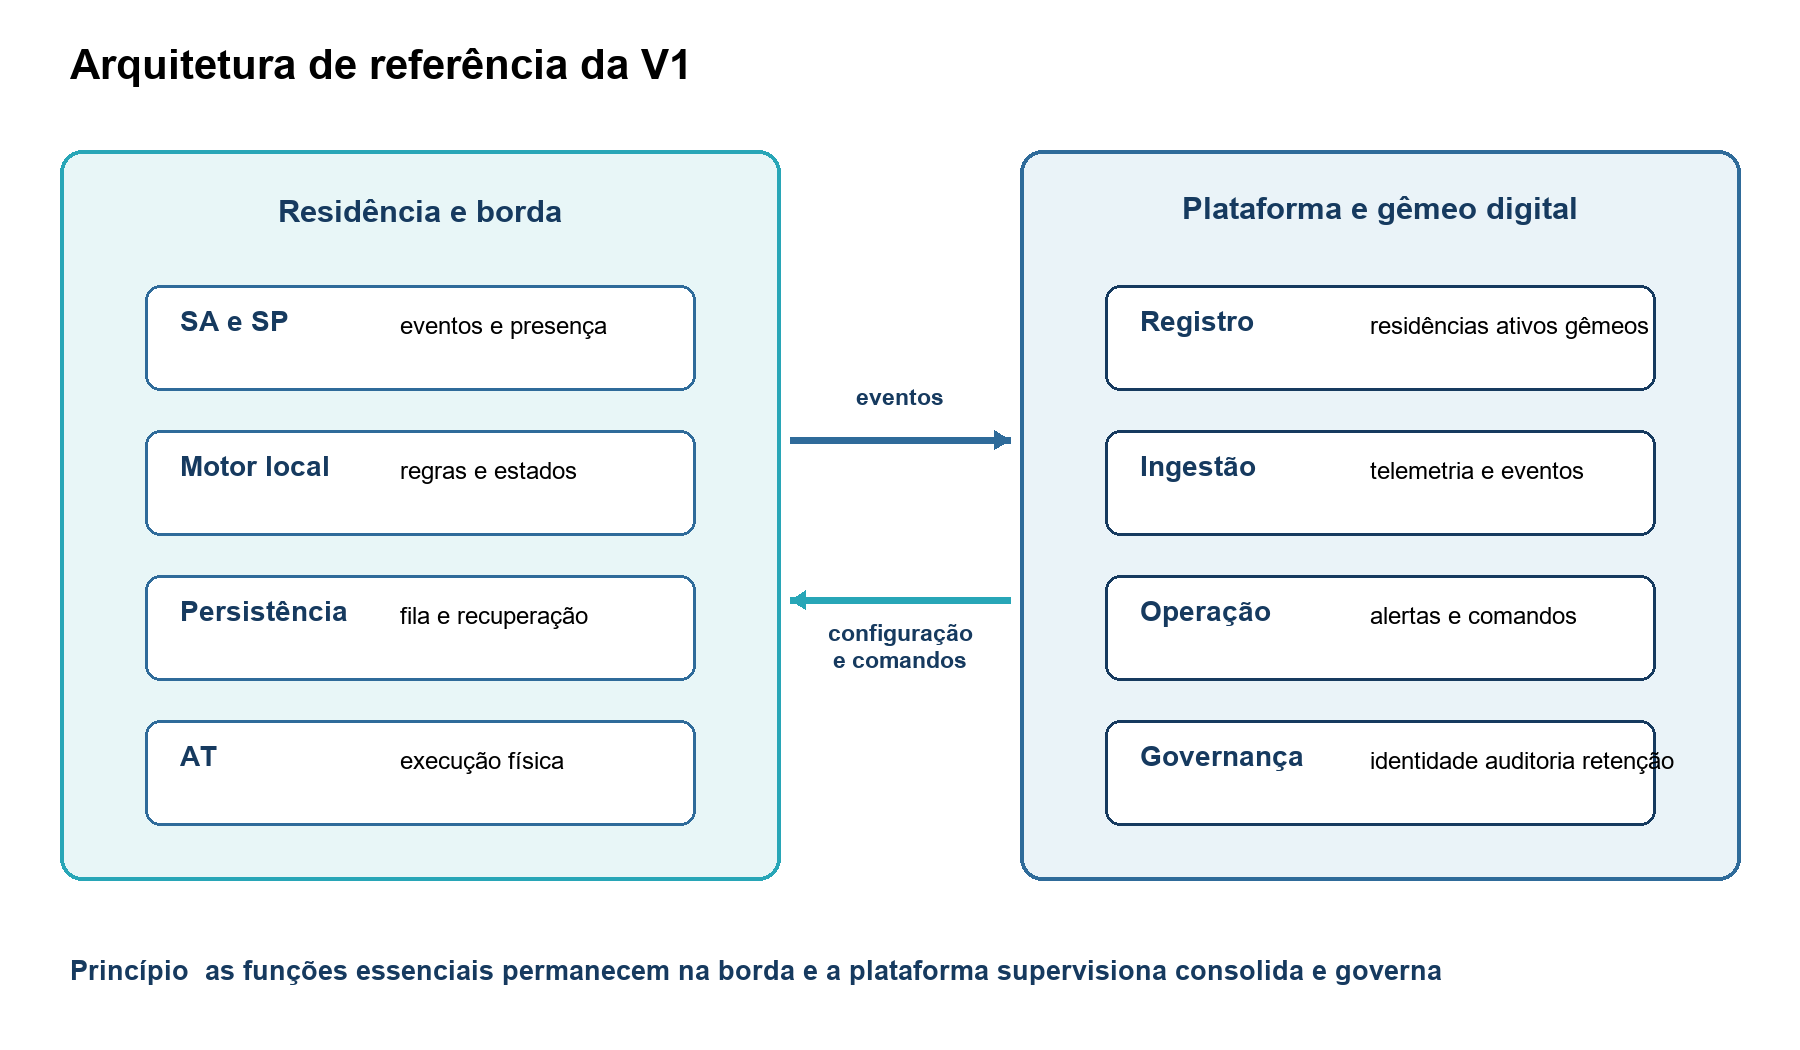
\includegraphics[width=0.88\linewidth]{images/apendice-arquitetura-v1.png}
\caption{Arquitetura de referência da V1: autonomia na borda e supervisão na plataforma.}
\label{fig:ap-arquitetura}
\end{figure}

A implementação separa núcleo e versões. O núcleo contém simulador, Hub, canal, Digital Twins, avaliação e gerador de cenários. Cada versão contém planta, roteiros, resultados esperados, controladores, documentação e dados. Entradas JSON são validadas por esquemas; o manifesto liga os CSVs ao código e às entradas. O ciclo completo é mostrado na Figura~\ref{fig:ciclo}.

\begin{figure}[ht]
\centering
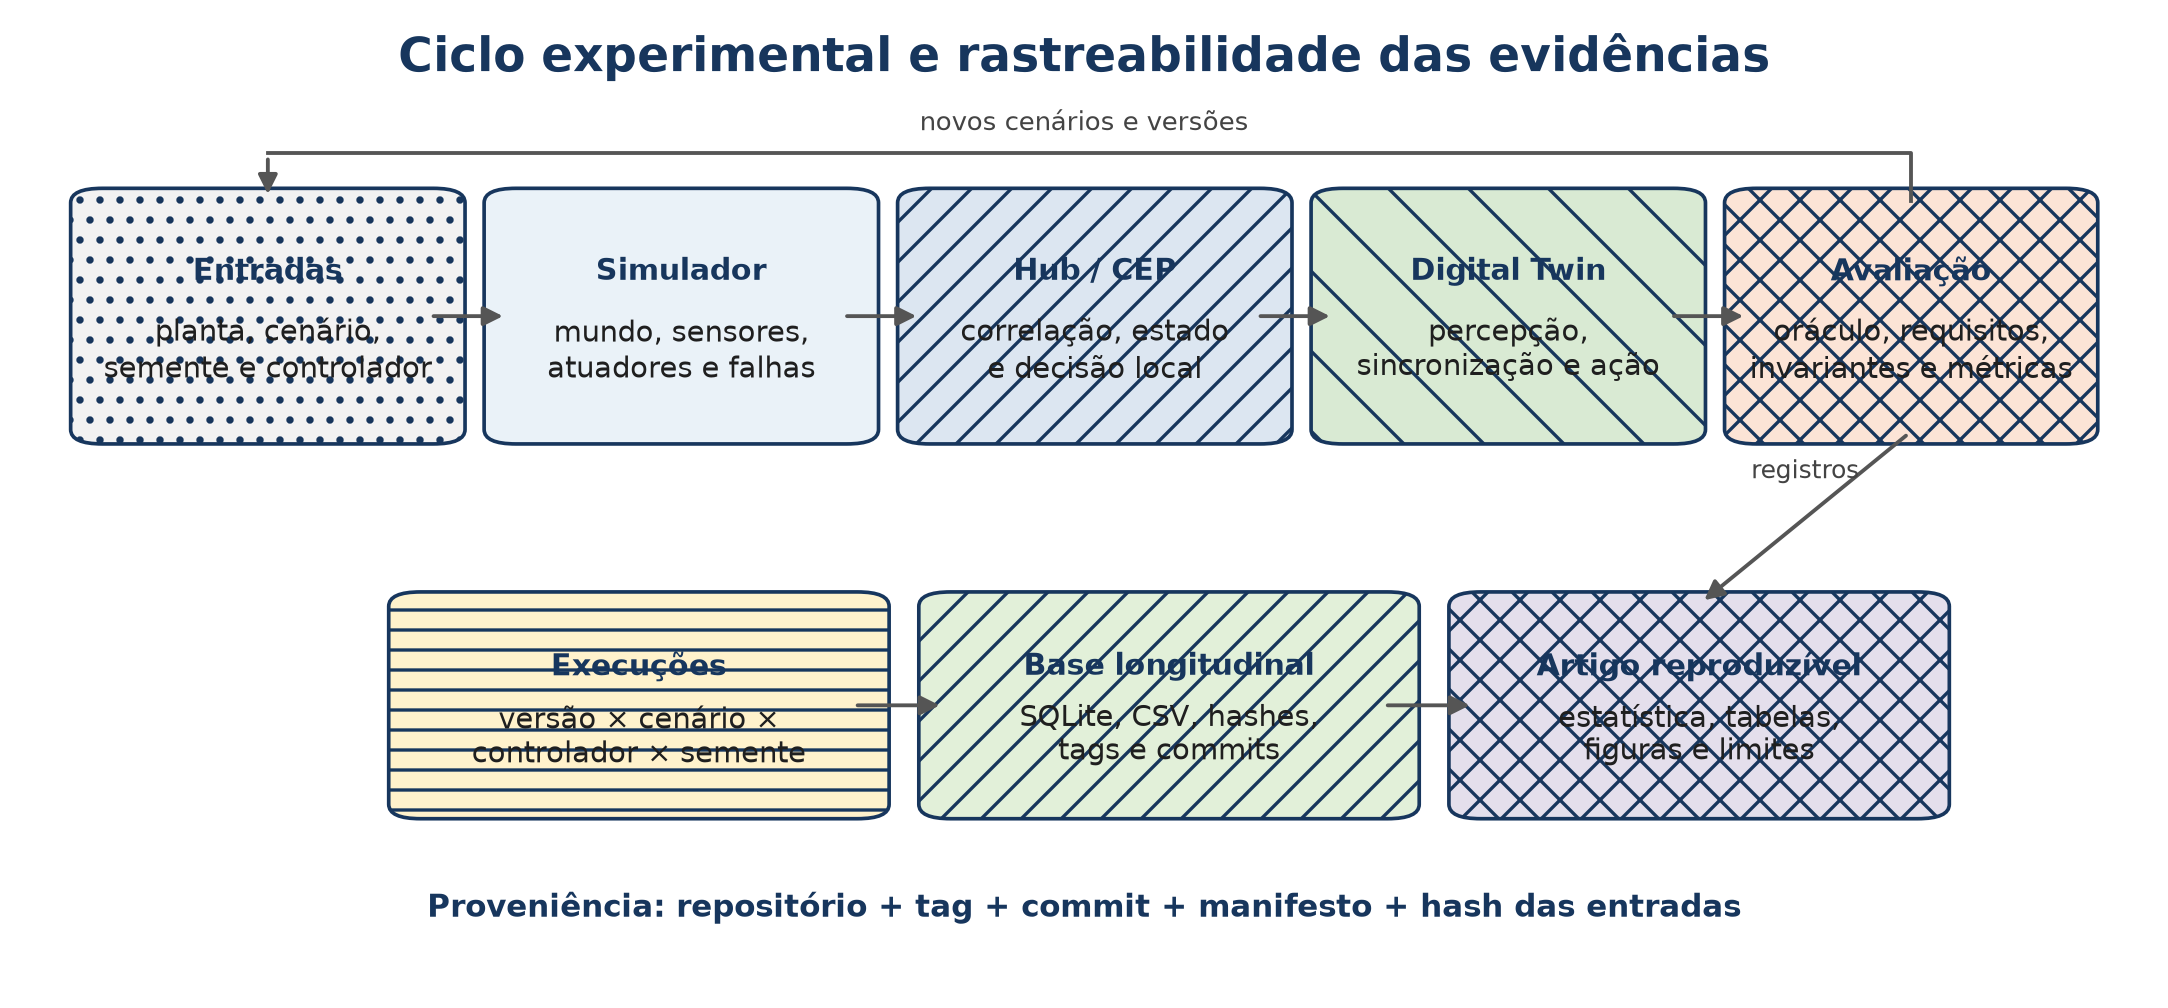
\includegraphics[width=0.90\linewidth]{images/figura-2-ciclo-experimental.png}
\caption{Ciclo versionado de construção, execução, análise e reprodução.}
\label{fig:ciclo}
\end{figure}

\begin{table}[ht]
\centering
\caption{Objetos principais da implementação e evidência associada.}
\small
\begin{tabularx}{\linewidth}{p{2.7cm}p{3.3cm}X}
\toprule
Objeto & Responsabilidade & Evidência reprodutível \\
\midrule
Planta e dispositivos & topologia, sensores e atuadores & JSON validado por esquema \\
Roteiro & eventos, tempos e resultado esperado & família e código do cenário \\
Controlador & decisão local de iluminação & referência ou grupo-exemplo \\
Hub e fila & percepção, autonomia e recuperação & entrega e reconciliação \\
Digital Twin & estado remoto e atualidade & divergência e fidelidade \\
Manifesto & proveniência da rodada & tags, commits, sementes e hashes \\
\bottomrule
\end{tabularx}
\end{table}

\subsection{Cenários, métricas e cadeia de evidências}

O protocolo transforma uma decisão arquitetural em evidência por uma cadeia rastreável: motivação, processo, capacidade, requisito, pacote de implementação, teste e resultado de aceite (Figura~\ref{fig:ap-rastreabilidade}). A unidade de análise não é a tela isolada nem um log sem contexto, mas a combinação versionada entre cenário, controlador e semente.

\begin{figure}[ht]
\centering
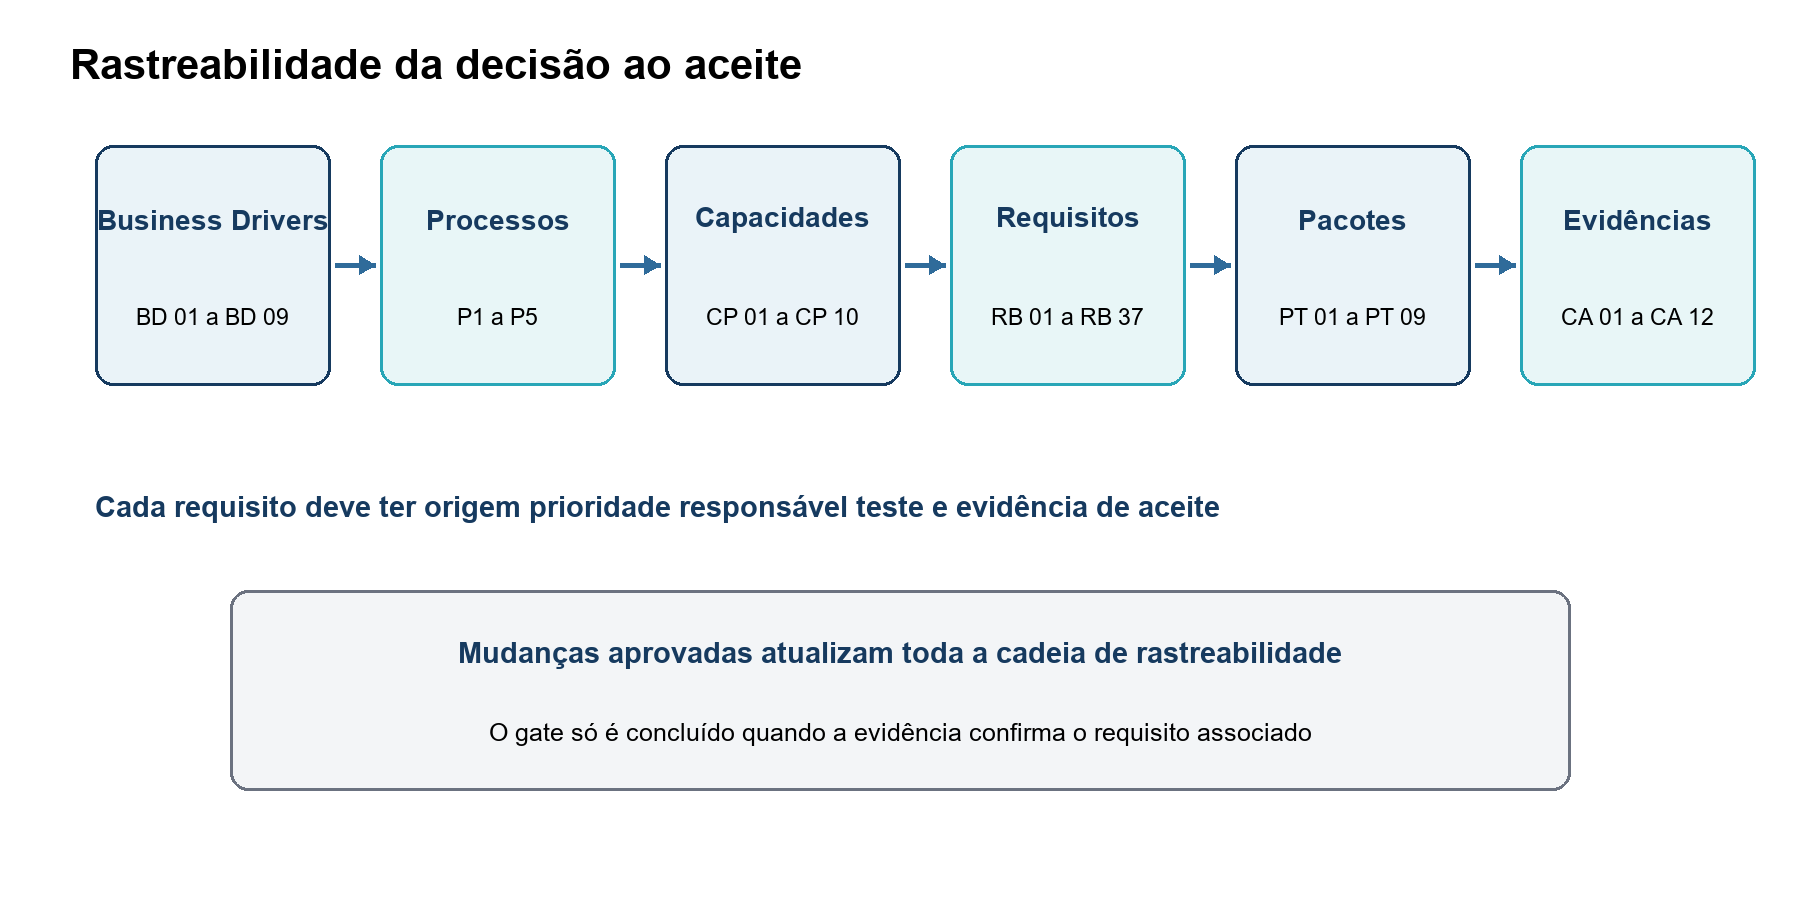
\includegraphics[width=0.90\linewidth]{images/apendice-rastreabilidade.png}
\caption{Cadeia de rastreabilidade entre decisão, implementação, teste e evidência.}
\label{fig:ap-rastreabilidade}
\end{figure}

Os cenários de destaque incluem N01, fluxo normal; FN01, falso negativo por imobilidade; DT05, partição de rede; DT08, decomposição entre percepção e sincronização; M01 e M12, circulação multiambiente; M05, falso negativo multiambiente; e M14, passagem sem direção observável. Eles exercitam reação, conforto, desperdício, ocupação desconhecida, atualidade, fila, reconciliação e fidelidade topológica.

\begin{figure}[ht]
\centering
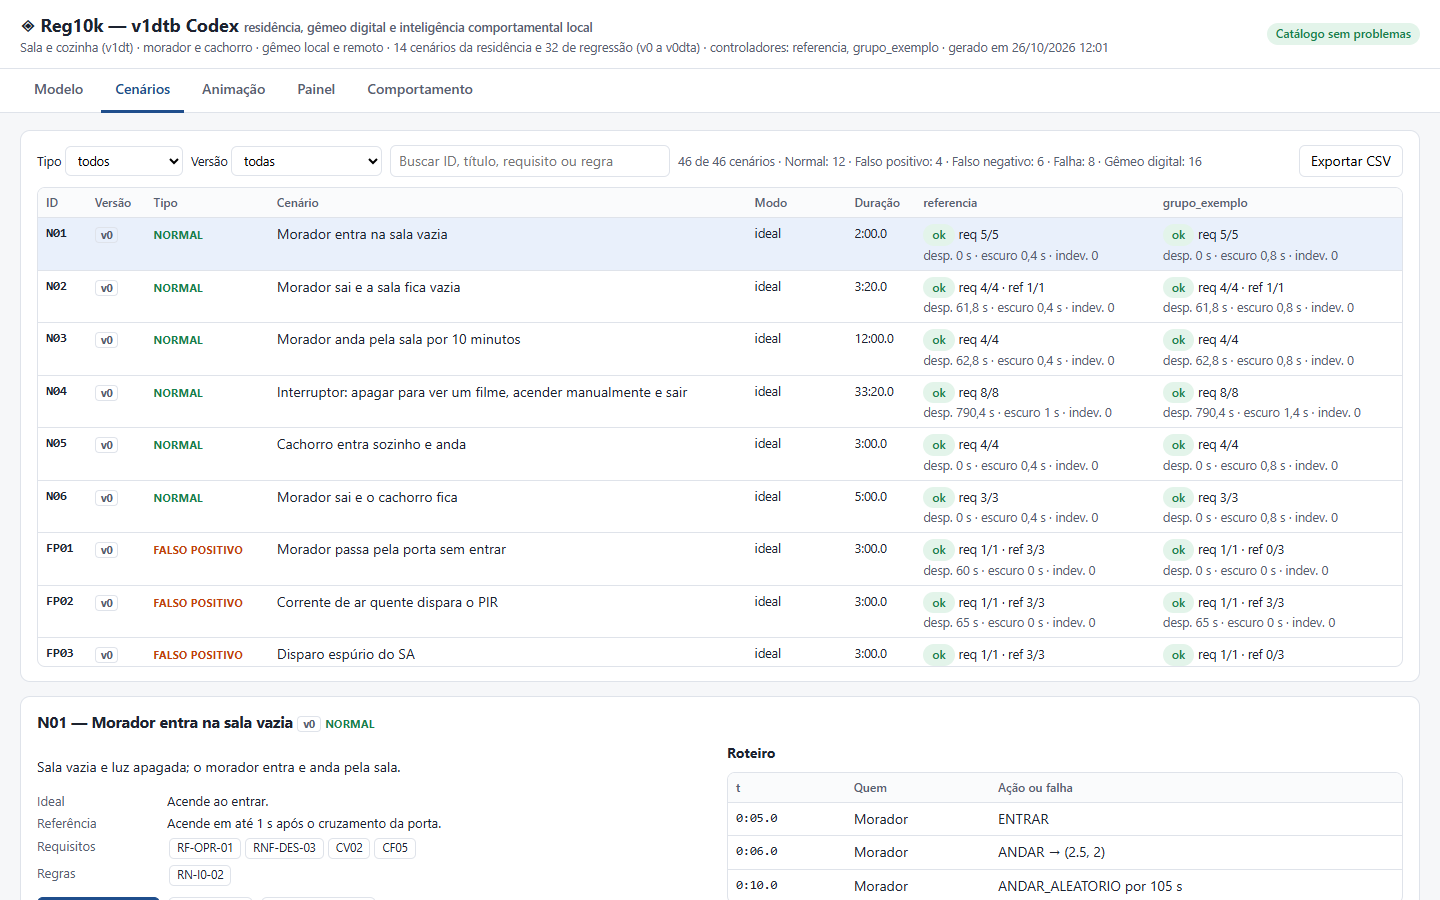
\includegraphics[width=0.96\linewidth]{images/tela-catalogo-cenarios.png}
\caption{Catálogo e seleção de cenários do simulador Reg10k. Os cards e a tabela relacionam versão, família, provocação, controlador, roteiro e requisitos, permitindo repetir uma situação sob configurações comparáveis.}
\label{fig:tela-cenarios}
\end{figure}

A análise usa semente mestre 5039 e 5.000 reamostragens. O manifesto registra 5.580 execuções, 2.790 pares e os derivados de atendimento, discordâncias, comparações contínuas, semântica de nulos e zeros e resumos por família. Planejamento e observação ficam separados para impedir que a v1dt.1 seja contada antes da execução.

\subsection{Roteiro de navegação e inspeção do sistema}

A navegação liga o efeito visível à causa técnica. O painel inicial apresenta cards de cenários; a seleção abre roteiro, planta e controlador. Durante a execução, o observador acompanha mundo simulado, percepção do Hub, Digital Twin remoto, espelho, linha do tempo e métricas. Fragmentos de rota permitem retornar à mesma evidência, por exemplo \texttt{\#cenarios/N01/referencia}.

\begin{figure}[ht]
\centering
\begin{minipage}[t]{0.49\linewidth}
\centering
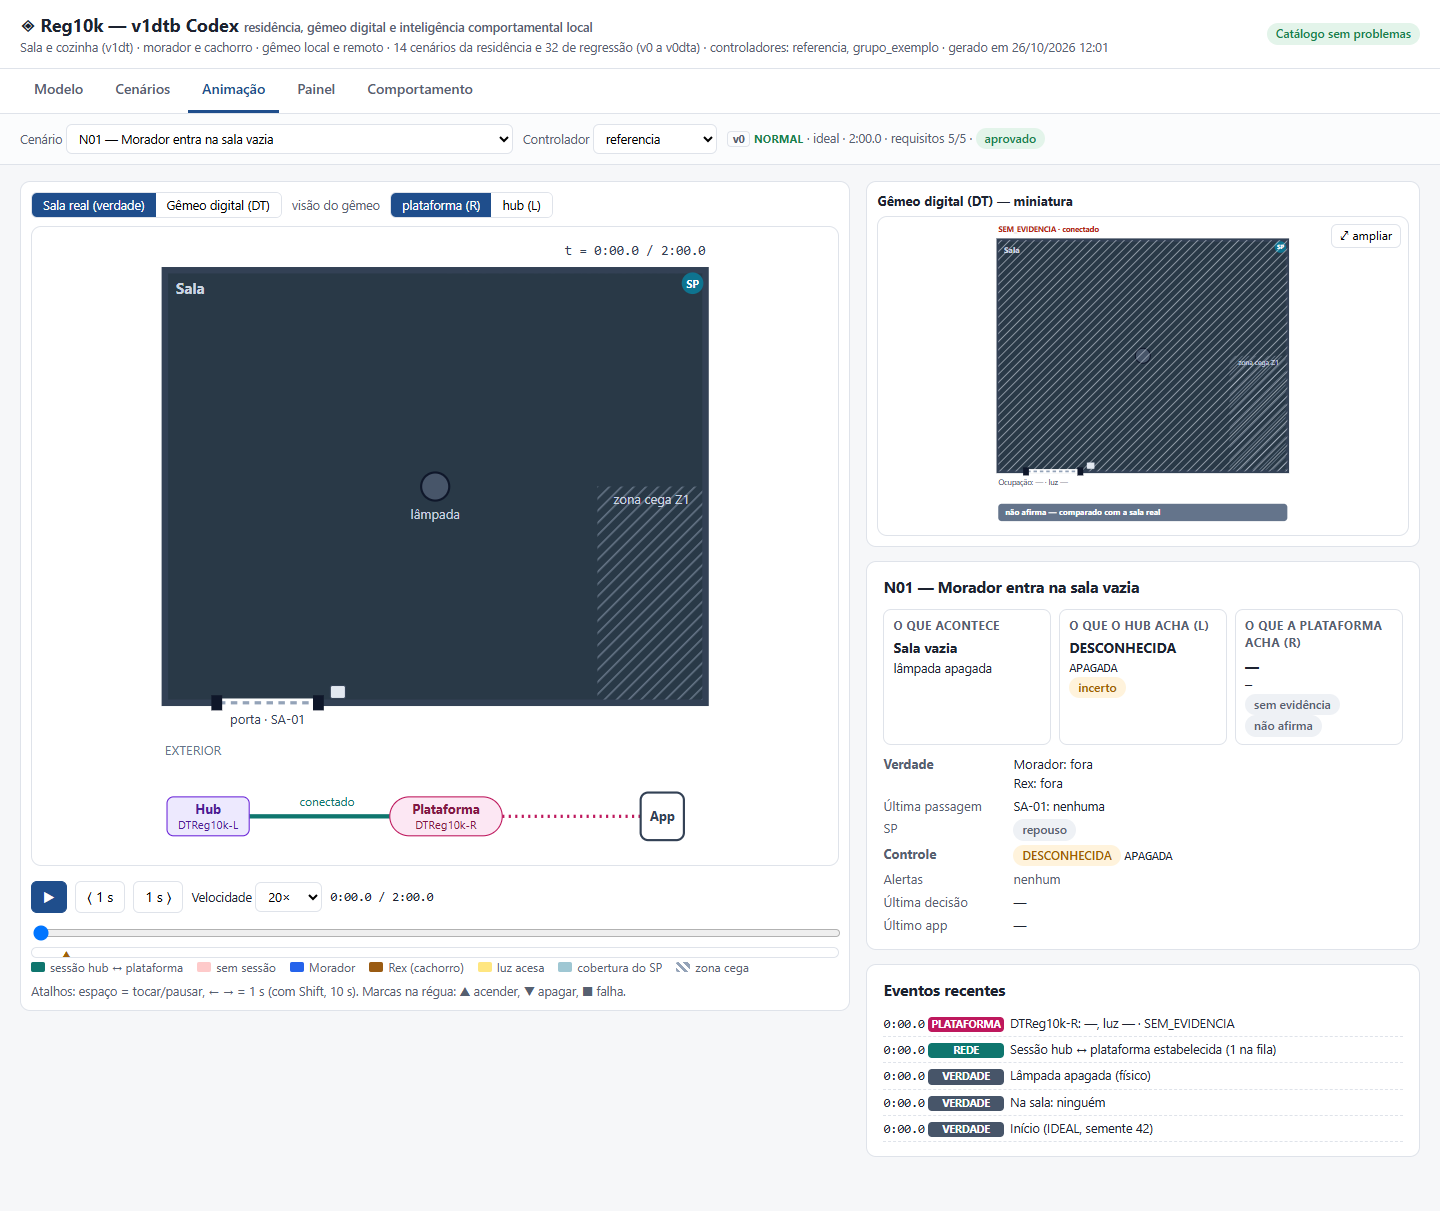
\includegraphics[width=\linewidth]{images/tela-animacao-n01.png}\\[-0.2ex]
\small (a) Animação, estado físico e representações digitais.
\end{minipage}\hfill
\begin{minipage}[t]{0.49\linewidth}
\centering
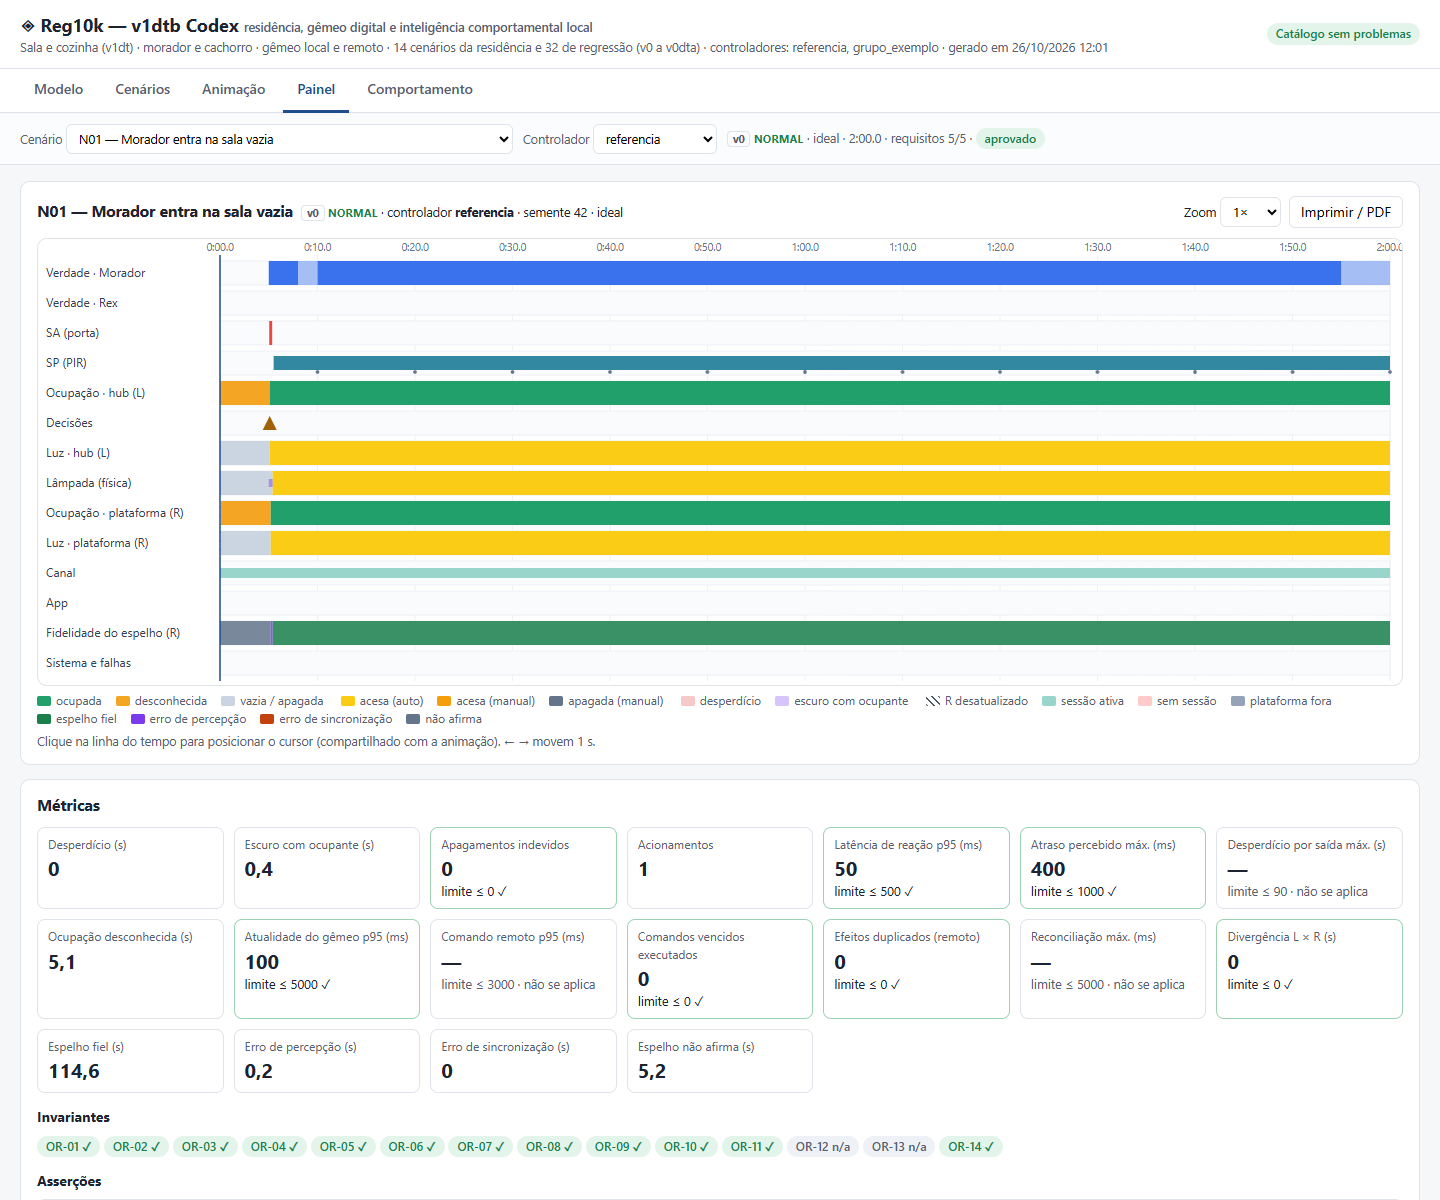
\includegraphics[width=\linewidth]{images/tela-painel-n01.png}\\[-0.2ex]
\small (b) Linha do tempo, métricas e verificações.
\end{minipage}
\caption{Inspeção do cenário N01 com controlador de referência e semente 42. A animação separa mundo, percepção do Hub e estado remoto; o painel liga os eventos às métricas de energia, conforto, atualidade e fidelidade.}
\label{fig:telas-inspecao}
\end{figure}

\begin{table}[ht]
\centering
\caption{Sequência recomendada de inspeção na interface.}
\small
\begin{tabularx}{\linewidth}{p{0.8cm}p{3.1cm}X p{3.0cm}}
\toprule
Etapa & Região & Pergunta orientadora & Evidência \\
\midrule
1 & cards & qual fenômeno será provocado? & família, código e objetivo \\
2 & planta e roteiro & o que ocorre no mundo físico? & passagem, presença e ação \\
3 & estados do Hub & o que foi percebido? & ocupação e confiança \\
4 & gêmeo e espelho & o remoto representa o mundo? & atualidade e fidelidade \\
5 & linha do tempo & qual evento causou a decisão? & ordem, janela e correlação \\
6 & métricas & qual compromisso foi produzido? & energia, conforto e erros \\
\bottomrule
\end{tabularx}
\end{table}

O roteiro evita interpretar a animação como evidência suficiente. Uma conclusão somente é aceita quando a sequência visível concorda com requisitos, invariantes, métricas e manifesto.

\subsection{Reprodutibilidade, versões e proveniência}

\begin{table}[ht]
\centering
\caption{Versões observadas e massa experimental.}
\label{tab:versoes}
\small
\begin{tabular}{llrrrr}
\toprule
Versão & Tag & Cômodos & Cenários & Execuções & Req. ref./grupo (\%) \\
\midrule
V0 & \texttt{v0dtb} & 1 & 38 & 2.280 & 100,00/100,00 \\
V1 & \texttt{v1dtc} & 2 & 26 & 1.560 & 99,87/89,87 \\
V2 & \texttt{v2dta} & 4 & 29 & 1.740 & 100,00/68,05 \\
\bottomrule
\end{tabular}
\end{table}

O núcleo está congelado na tag \texttt{nucleo-v1.2}; as massas estão nas tags da Tabela~\ref{tab:versoes} \citep{reg10ksoftware}. Um repositório distinto preserva scripts, SQLite, CSVs derivados, planilha, testes e manuscrito \citep{reg10krepro}. A combinação repositório--tag--commit--hash permite reconstruir a configuração enquanto os ramos principais continuam evoluindo.

\section{Evolução da arquitetura com Gêmeo Digital}

\subsection{Automação local e isolada}

O ponto de partida encerra estado e decisão na residência. Sensores detectam passagem e presença, o controlador decide e o atuador comanda a lâmpada. O log local registra fatos, mas não mantém uma representação compartilhada, não correlaciona residências e não oferece supervisão de plataforma.

\subsection{V0: estado digital de um cômodo}

A V0 acrescenta Hub, Digital Twin e espelho, separando mundo, percepção, sincronização e decisão. Torna-se possível medir não apenas se a lâmpada acendeu, mas se o sistema sabia que o cômodo estava ocupado e por quanto tempo representou estado incorreto.

\subsection{V1: correlação espacial}

A V1 introduz cozinha e passagem interna. A transição muda origem e destino, embora os sensores não revelem direção ou identidade. A decisão depende de correlacionar passagem, presença e estado anterior; o gêmeo passa a representar uma pequena topologia residencial.

\subsection{V2: escala residencial}

A V2 expande a planta para quatro cômodos. Parâmetros variam por ambiente, a cobertura manual torna-se frágil e a geração sistemática de cenários ganha importância. O crescimento também exige normalização: totais de eventos, desperdício ou divergência não são comparáveis sem considerar cômodos, ocupação e famílias.

\subsection{v1dt.1: ocupação, comportamento e intenção}

A evolução planejada mantém a planta da V1 e altera a população. Múltiplos moradores, criança, idoso, visitante e cachorro produzem movimentos distintos, mas sensores não fornecem identidade ou intenção. Ler e dormir podem gerar a mesma ausência de movimento e demandar decisões opostas. O gêmeo deve representar incerteza, origem da evidência e possibilidade de revisão.

\begin{figure}[ht]
\centering
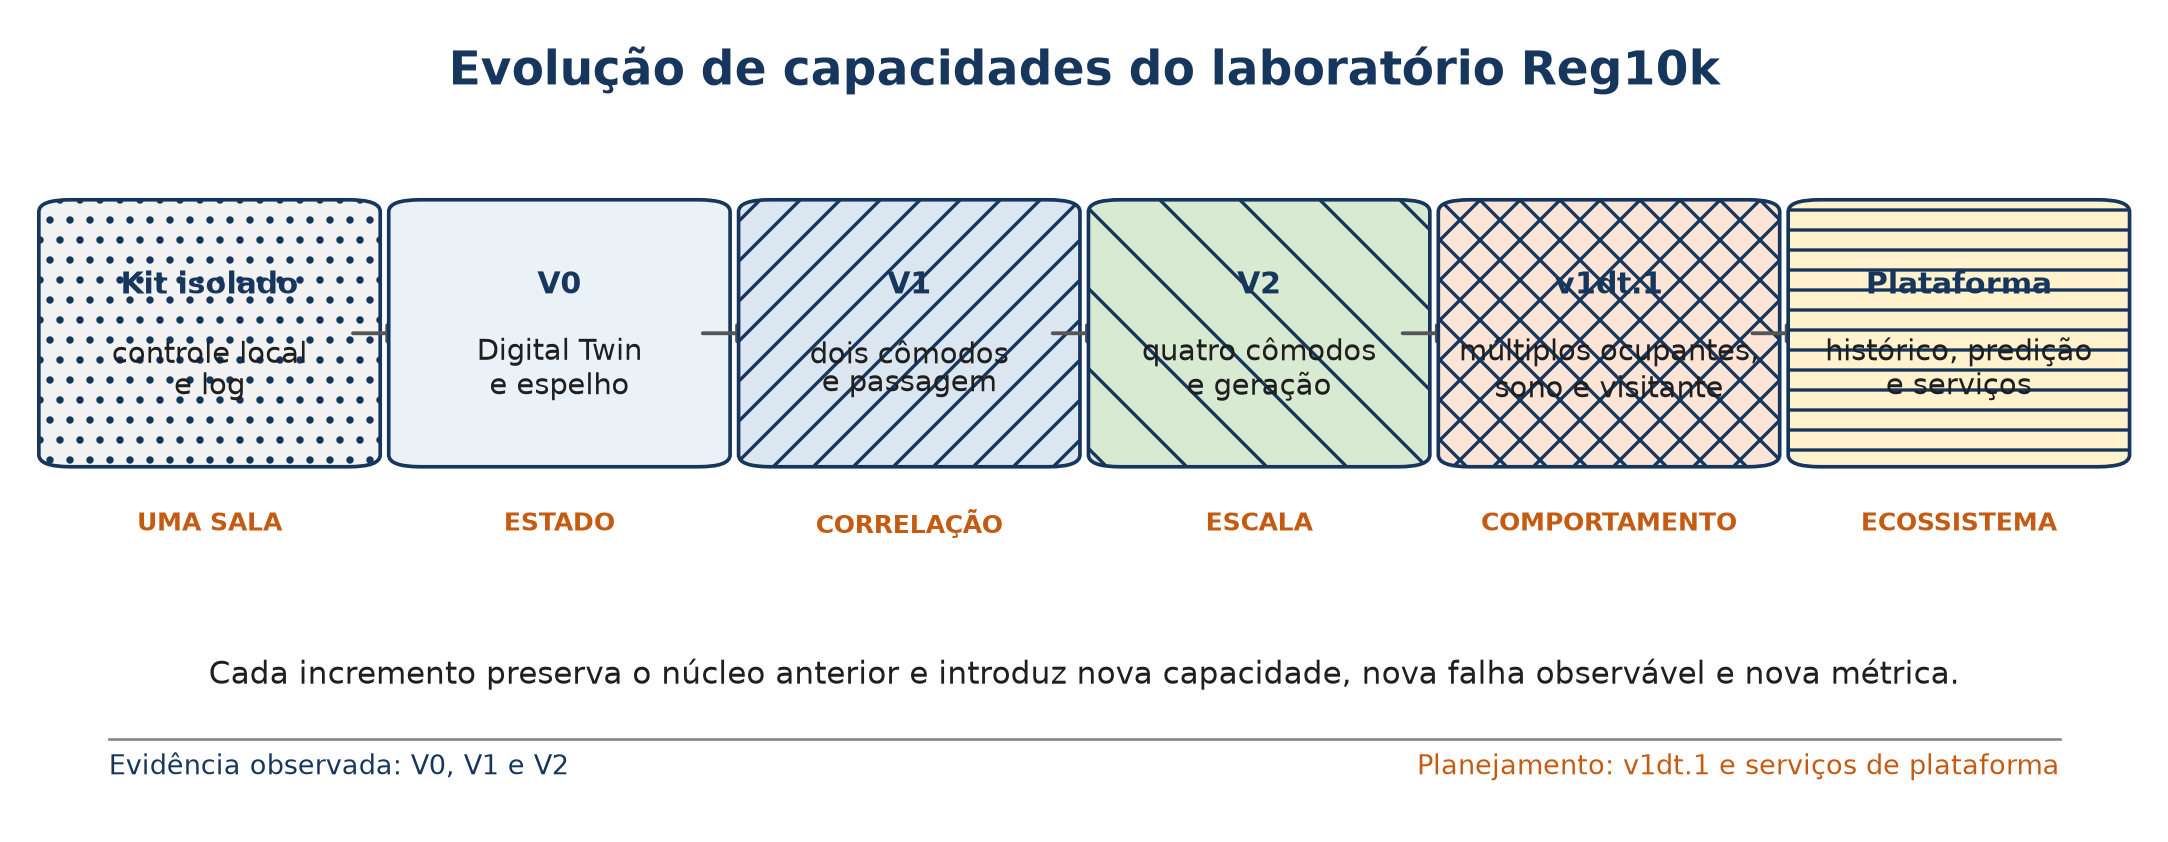
\includegraphics[width=0.94\linewidth]{images/figura-1-evolucao-capacidades.png}
\caption{Evolução incremental das capacidades do Reg10k.}
\label{fig:evolucao}
\end{figure}

\subsection{Da residência conectada à plataforma}

Quando residências são conectadas, eventos derivados podem apoiar recomendação energética, previsão de carga, identificação de falhas e alertas graduados. São possibilidades arquiteturais, não resultados deste experimento. Dependem de consentimento, qualidade, segurança, governança e modelos de responsabilidade.

\section{O laboratório na PCS5039}

O encadeamento evento $\rightarrow$ CEP $\rightarrow$ Digital Twin $\rightarrow$ ação funciona como linguagem comum. Nos projetos, muda a entidade do gêmeo e a janela decisória, mas permanece a necessidade de correlacionar evidências, comparar estado presente com comportamento esperado e agir em tempo útil (Tabela~\ref{tab:transferencia}).

\begin{table}[ht]
\centering
\caption{Transferência do padrão arquitetural a projetos da disciplina.}
\label{tab:transferencia}
\small
\begin{tabularx}{\linewidth}{p{2.0cm}p{2.3cm}X p{2.1cm}}
\toprule
Domínio & Entidade & Situação derivada & Ação \\
\midrule
Pontes & estrutura & vibração e deformação crescentes & inspecionar/restringir \\
Apoio a idosos & pessoa/rotina & ausência de movimento ou resposta & verificar/alertar \\
CI/CD & pipeline & falha recorrente após alteração & bloquear/reverter \\
Veículo autônomo & veículo/entorno & obstáculo na distância de frenagem & frear/desviar \\
\bottomrule
\end{tabularx}
\end{table}

Essa transferência é evidência de reutilização conceitual, não de efetividade pedagógica. Uma avaliação posterior deverá usar rubrica comum para arquitetura, eventos, gêmeo e reprodutibilidade; comparar entregas iniciais e finais; e triangular artefatos, testes e percepção dos participantes.

\section{Resultados e discussão}

\subsection{Cobertura e aumento de complexidade}

Todos os 5.580 registros satisfizeram os invariantes avaliados. O controlador de referência atendeu aos requisitos em 100\%, 99,87\% e 100\% das execuções de V0, V1 e V2; o grupo-exemplo, em 100\%, 89,87\% e 68,05\%. Na V1, 701 pares tiveram ambos aprovados, 78 somente a referência e um ambos reprovados. Na V2, foram 592 pares com ambos aprovados e 278 somente referência; nenhum teve apenas o grupo aprovado. O aumento da topologia expôs limitações invisíveis no caso simples, enquanto a preservação de invariantes separou integridade do ambiente e adequação funcional.

\subsection{Escala, normalização e compromissos}

No controlador de referência, a média de eventos por execução foi 1.073,13 na V0, 1.044,33 na V1 e 2.021,11 na V2. Por cômodo, tornou-se 1.073,13, 522,17 e 505,28. A queda normalizada não prova eficiência, pois versões diferem em cenários e famílias; demonstra que totais brutos confundem escala, cobertura e comportamento.

O desperdício médio de referência cresceu de 56,61 s para 93,58 s e 155,23 s; por cômodo, caiu de 56,61 s para 46,79 s e 38,81 s. O tempo médio no escuro foi 105,84 s, 39,11 s e 45,30 s; por cômodo, 105,84 s, 19,56 s e 11,32 s. Medianas menores que médias indicam muitos casos sem ocorrência e poucos com cauda longa.

No pareamento da V2, o grupo reduziu desperdício em 12,37 s (IC95: $-26{,}75$; $-2{,}07$), mas aumentou o tempo no escuro com ocupante em 1,41 s (IC95: 1,02; 1,85) e reduziu a fidelidade em 0,08 ponto percentual (IC95: $-0{,}11$; $-0{,}06$). Portanto, existe compromisso entre energia, conforto e representação, e não superioridade geral.

\subsection{Fidelidade do Digital Twin}

A fidelidade média de referência foi 59,94\% na V0, 62,27\% na V1 e 55,92\% na V2. Como inclui cenários de falha e desconexão, não é uma nota global. O erro médio de percepção foi 127,68 s, 99,42 s e 175,08 s; o de sincronização, 0,016 s, 0,004 s e zero. Nos parâmetros simulados, a divergência decorre sobretudo do que o Hub infere, não do transporte até a plataforma. Conectar percepção incorreta apenas distribui o erro com maior rapidez.

\begin{table}[ht]
\centering
\caption{Evidências, interpretações permitidas e limites.}
\label{tab:evidencias}
\small
\begin{tabularx}{\linewidth}{p{3.5cm}X p{3.5cm}}
\toprule
Evidência & Interpretação & Limite \\
\midrule
5.580 execuções; 2.790 pares & protocolo executável e pareado & simulação, não campo \\
100\% de invariantes & integridade estrutural preservada & invariantes disponíveis \\
V2: desperdício $-12{,}37$ s & grupo usa menos luz no conjunto & cenários observados \\
V2: escuro $+1{,}41$ s & troca energia por conforto & sem superioridade geral \\
Percepção $\gg$ sincronização & limite sensorial domina o modelo & rede simulada \\
Quatro domínios discentes & transferência do padrão & sem efeito causal \\
\bottomrule
\end{tabularx}
\end{table}

As respostas às RQs são parciais e delimitadas. Para RQ1, versões ligam capacidade nova a problema observável sob protocolo comum. Para RQ2, medidas precisam ser estratificadas e normalizadas. Para RQ3, o gêmeo torna mensuráveis percepção, sincronização, atualidade e incerteza. Para RQ4, há transferência estrutural, ainda sem mensuração causal de aprendizagem.

\section{Conclusão}

O Reg10k transforma uma automação de iluminação em laboratório de arquitetura orientada a eventos e Digital Twins. Seu valor não está na quantidade de dispositivos, mas na separação verificável entre mundo, percepção, sincronização e decisão. A progressão V0--V2 mostrou que complexidade espacial expõe falhas ocultas e que métricas brutas podem conduzir a interpretações inadequadas. O pareamento revelou compromissos entre desperdício, conforto e fidelidade; a decomposição do erro mostrou predominância da percepção no modelo.

A contribuição educacional é um caminho reproduzível para discutir decisões arquiteturais com evidência. O próximo experimento, v1dt.1, avaliará ocupação múltipla, sono, presença incompatível, precisão, revocação e conciliação. Estudos futuros devem executar o ambiente em campo, ampliar controladores e medir aprendizagem com instrumentos independentes. As referências autorais foram deliberadamente trianguladas com pelo menos duas fontes conceituais independentes por tema, reduzindo polarização e tornando explícita a linhagem teórica das escolhas.

\begin{thebibliography}{99}
\small
\bibitem[Arakaki(2026a)]{reg10ksoftware} ARAKAKI, R. \textit{PCS5039 ambiente Reg10k: núcleo e versões experimentais}. GitHub, 2026. Disponível em: \repoReg. Acesso em: 29 out. 2026.
\bibitem[Arakaki(2026b)]{reg10krepro} ARAKAKI, R. \textit{PCS5039 Reg10k: artigo e pacote de reprodutibilidade}. GitHub, 2026. Disponível em: \repoArt. Acesso em: 29 out. 2026.
\bibitem[Barker et al.(2022)]{barker2022} BARKER, M. et al. Introducing the FAIR Principles for research software. \textit{Scientific Data}, v. 9, art. 622, 2022. DOI: \href{https://doi.org/10.1038/s41597-022-01710-x}{10.1038/s41597-022-01710-x}.
\bibitem[Brandão et al.(2026)]{brandao2026} BRANDÃO, L.; ARAKAKI, R.; SILVA, J. Educational Digital Twins modeled with RM-ODP for closed-loop supervision. \textit{SSRN}, 2026. DOI: \href{https://doi.org/10.2139/ssrn.6631129}{10.2139/ssrn.6631129}.
\bibitem[Coombs et al.(2026)]{coombs2026} COOMBS, C.; SOBAN, D.; MCCARTAN, C. Learning outcomes of Digital Twins in engineering education: a systematised review. In: \textit{22nd International CDIO Conference}. Reykjavik, 2026.
\bibitem[Cugola e Margara(2012)]{cugola2012} CUGOLA, G.; MARGARA, A. Processing flows of information: from data stream to complex event processing. \textit{ACM Computing Surveys}, v. 44, n. 3, art. 15, 2012. DOI: \href{https://doi.org/10.1145/2187671.2187677}{10.1145/2187671.2187677}.
\bibitem[Fujii et al.(2022)]{fujii2022} FUJII, Y. et al. A Digital Twin architecture for smart residential energy management with MLOps. \textit{Machines}, v. 10, n. 1, art. 23, 2022. DOI: \href{https://doi.org/10.3390/machines10010023}{10.3390/machines10010023}.
\bibitem[Harris et al.(2026)]{harris2026} HARRIS, J.; KITTUR, J.; CARTER, V. Digital twin technology in engineering education: a systematic review. \textit{Frontiers in Education}, v. 11, 2026. DOI: \href{https://doi.org/10.3389/feduc.2026.1955212}{10.3389/feduc.2026.1955212}.
\bibitem[Hevner et al.(2004)]{hevner2004} HEVNER, A. et al. Design science in information systems research. \textit{MIS Quarterly}, v. 28, n. 1, p. 75--105, 2004. DOI: \href{https://doi.org/10.2307/25148625}{10.2307/25148625}.
\bibitem[ISO(1998)]{iso10746} ISO. \textit{ISO/IEC 10746-1:1998: Information technology --- Open Distributed Processing --- Reference model: Overview}. Geneva, 1998.
\bibitem[ISO(2023)]{iso25010} ISO. \textit{ISO/IEC 25010:2023: Systems and software engineering --- Product quality model}. Geneva, 2023.
\bibitem[ISO/IEC/IEEE(2022)]{iso42010} ISO/IEC/IEEE. \textit{42010:2022: Software, systems and enterprise --- Architecture description}. Geneva, 2022.
\bibitem[Katz et al.(2021)]{katz2021} KATZ, D.; GRUENPETER, M.; HONEYMAN, T. Taking a fresh look at FAIR for research software. \textit{Patterns}, v. 2, n. 3, art. 100222, 2021. DOI: \href{https://doi.org/10.1016/j.patter.2021.100222}{10.1016/j.patter.2021.100222}.
\bibitem[Kritzinger et al.(2018)]{kritzinger2018} KRITZINGER, W. et al. Digital Twin in manufacturing: a categorical literature review and classification. \textit{IFAC-PapersOnLine}, v. 51, n. 11, p. 1016--1022, 2018. DOI: \href{https://doi.org/10.1016/j.ifacol.2018.08.474}{10.1016/j.ifacol.2018.08.474}.
\bibitem[Luckham(2002)]{luckham2002} LUCKHAM, D. \textit{The Power of Events: An Introduction to Complex Event Processing in Distributed Enterprise Systems}. Boston: Addison-Wesley, 2002.
\bibitem[Peffers et al.(2007)]{peffers2007} PEFFERS, K. et al. A design science research methodology for information systems research. \textit{Journal of Management Information Systems}, v. 24, n. 3, p. 45--77, 2007. DOI: \href{https://doi.org/10.2753/MIS0742-1222240302}{10.2753/MIS0742-1222240302}.
\bibitem[Saad e Arakaki(2014)]{saad2014} SAAD, S.; ARAKAKI, R. An event processing architecture for continuous operational risk barrier monitoring. In: \textit{8th ACM International Conference on Distributed Event-Based Systems}. 2014. DOI: \href{https://doi.org/10.1145/2611286.2611307}{10.1145/2611286.2611307}.
\bibitem[Smith et al.(2016)]{smith2016} SMITH, A. et al. Software citation principles. \textit{PeerJ Computer Science}, v. 2, e86, 2016. DOI: \href{https://doi.org/10.7717/peerj-cs.86}{10.7717/peerj-cs.86}.
\bibitem[Tao et al.(2019)]{tao2019} TAO, F. et al. Digital Twins and cyber--physical systems toward smart manufacturing and Industry 4.0: correlation and comparison. \textit{IEEE Transactions on Industrial Informatics}, v. 15, n. 4, p. 2405--2415, 2019. DOI: \href{https://doi.org/10.1109/TII.2018.2873186}{10.1109/TII.2018.2873186}.
\bibitem[Wilkinson et al.(2016)]{wilkinson2016} WILKINSON, M. et al. The FAIR Guiding Principles for scientific data management and stewardship. \textit{Scientific Data}, v. 3, art. 160018, 2016. DOI: \href{https://doi.org/10.1038/sdata.2016.18}{10.1038/sdata.2016.18}.
\end{thebibliography}
\end{document}
